\documentclass[11pt]{article}
\usepackage[final]{acl}
\usepackage{times}
\usepackage{latexsym}
\usepackage[T1]{fontenc}
\usepackage[utf8]{inputenc}
\usepackage{microtype}
\usepackage{inconsolata}
\usepackage{graphicx}
\usepackage{booktabs}
\usepackage{amsmath,amssymb,amsthm}
\usepackage{xcolor}
\newtheorem{proposition}{Proposition}
\newtheorem{observation}{Observation}
\newcommand{\pL}{\texttt{\textbackslash p\{L\}}}
\newcommand{\pM}{\texttt{\textbackslash p\{M\}}}
\newcommand{\RO}{\textsc{R0}}
\newcommand{\RI}{\textsc{R1}}
\newcommand{\RII}{\textsc{R2}}

\title{Extend or Repair? Vocabulary Extension Cannot Cross\\ a Pre-Tokenizer Boundary}

\author{Aarjan Chaudhary \and Shrey Sharma \and Navyata Dhakal \\
  Independent researchers, Nepal \\
  \texttt{arjanchaudharyy@gmail.com}}

\begin{document}
\maketitle

\begin{abstract}
Llama-3, Qwen3 and many other open LLMs pre-tokenize text with a regular expression whose word class admits only Unicode letters. Devanagari vowel signs are combining marks, so this regex splits Nepali words at every vowel sign, and models that use it spend $2.6$ to $5.8$ times as many tokens on Nepali as on the same English text. Merge-based vocabulary extension cannot join the split pieces: for Llama-3 and Qwen3 no number of new merges brings this premium below about $2.2$, and ten released extensions already end within 4\% of this pre-token floor. We give a small edit to the deployed regex that provably keeps every token id of text without combining marks or Devanagari characters. With 32{,}000 new merges it brings Nepali to $1.01$ times English, about 54\% fewer Nepali tokens than standard extension. In small-budget continued pretraining of Llama-3.2-1B and Qwen3-0.6B, the original tokenizer gave the lowest held-out Nepali bits per byte under every recipe we tested. Matching the repair's training steps to standard extension, with about 35\% of the data repeated, reversed their order on Qwen but not on Llama. Whether the token savings give a favourable latency and quality trade-off in generation remains untested. We release the tokenizers and code.
\end{abstract}

\section{Introduction}

On parallel FLORES-200 text, Qwen3's tokenizer needs $4.42$ times as many tokens for a Nepali sentence as for its English translation, and the \texttt{cl100k} tokenizer used by Phi-4, OLMo-2 and Granite-4.1 needs $4.76$ times as many (\S\ref{sec:audit}). We call this ratio the \emph{premium}. Nepali speakers pay it on every request, in price, latency and usable context.

Much of the premium has a mechanical cause. GPT-2-style pre-tokenizers split text with a regular expression whose word class \pL{} matches one or more Unicode letters~\citep{gpt2encoder}; we call it the \emph{letters-only regex}. In Unicode, Devanagari vowel signs, the virama, the anusvara and the candrabindu are combining marks (\pM{}), so the regex starts a new pre-token at each of them and byte-pair encoding (BPE) can never merge across that boundary. \citet{regmi2026vowel} identified this cause and the resulting bound on token counts. They showed that adding marks to the word class cuts Nepali from 4.78 to 1.58 tokens per word, and that 63\% of the 1{,}345 text-generation repositories they examined still use the letters-only class.

Regmi et al.\ studied tokenizers trained from scratch. Most practitioners instead adapt a model that already exists, usually by vocabulary extension: they add target-language tokens, initialise their embeddings and continue pretraining~\citep{tejaswi-etal-2024-exploring,yamaguchi2026lowres,purason-etal-2026-teaching,smith2026inplace}. What is new in this paper is that deployed-model setting. We show that the bound becomes a floor that released merge-based extensions already hit; we give a repair of a deployed model's regex that provably keeps English token ids; and we test it in controlled continued pretraining against the standard continued-BPE recipe of \citet{purason-etal-2026-teaching}, with the tokenizers released.

\paragraph{Findings.} For Llama-3 and Qwen3 the \emph{pre-token floor}, the lowest premium any merge-based extension can reach, is about $2.2$ (\S\ref{sec:floor}). Ten released extensions for six scripts end within 4\% of their floors, and our own extension under the letters-only regex stalls at it. Registering \RII{}'s learned strings as added tokens does get below the floor, but a fifth of the matches then start in the middle of a word. Our repair adds marks to the word class with two string substitutions and, together with new merges, brings Nepali to parity with English while leaving every token id of mark-free, non-Devanagari text unchanged (\S\ref{sec:method}). The model-quality result is less favourable. Under our pre-registered analysis, continued pretraining with no new tokens gave the best held-out Nepali bits per byte on both models, so our main hypothesis failed. Between the two extension recipes, the repair was non-inferior to standard extension for Llama and slightly worse for Qwen, and it was clearly worse for Llama when scored after the separator used in training (\S\ref{sec:cpt}). It needs about half as many decoding steps as standard extension for the same Nepali text.

\paragraph{Contributions.} We make four contributions:
\begin{enumerate}
  \setlength\itemsep{0pt}
  \item Evidence that the pre-token floor binds released merge-based extensions, and a test of the added-token route around it (\S\ref{sec:floor}); an audit of 24 distinct deployed tokenizers with per-tokenizer floors (\S\ref{sec:audit}).
  \item An English-preserving repair of a deployed regex with a proof, a Devanagari-only variant with a stronger guarantee, and a practical pitfall in loading repaired tokenizers (\S\ref{sec:method}).
  \item A pre-registered comparison of \RO{} (no extension), \RI{} (standard extension) and \RII{} (repair + extension) in continued pretraining of two deployed models, reported against the registered hypotheses (\S\ref{sec:cpt}).
  \item The tokenizers, code and analysis plan.\footnote{\artifactnote}
\end{enumerate}

\section{Related work}
\label{sec:related}

\paragraph{Tokenization premiums.} Tokenizers trained mostly on English encode other languages in more tokens, so those languages pay more for the same content~\citep{petrov2023unfairness,ahia-etal-2023-languages,lundin-etal-2026-token,ovcharov2026european,somide2026african,tamang2024evaluating}. For Nepali, \citet{kadariya2026nepali} report $4.79\times$ for \texttt{cl100k}. \citet{srivastava2026tokenizertax} and \citet{mandarapu2026ledger} measure large Indic premiums on FLORES-200, and the former reports that \texttt{o200k} cuts the mean Indic premium from $8.0\times$ to $2.1\times$, without attributing the change to the regex. We report sentence-level token ratios on parallel FLORES-200 text~\citep{goyal-etal-2022-flores,nllb2022}, following \citet{petrov2023unfairness}, with paired bootstrap intervals. Fewer tokens do not by themselves make a better model~\citep{schmidt-etal-2024-tokenization}, which is why we test the repair with continued pretraining.

\paragraph{Pre-tokenization of combining marks.} A 2024 tiktoken issue reported that GPT-2-style regexes split Indic words at vowel signs and proposed the word class \texttt{[\textbackslash p\{L\}\textbackslash p\{M\}]+}~\citep{tiktoken_issue292}. ZeTT~\citep{minixhofer2024zett} adjusted its GPT-2-based regex to avoid over-segmenting Hindi and Tamil. \citet{velayuthan-sarveswaran-2025-egalitarian} showed that the GPT-2, GPT-4 and Llama-3 pre-tokenizers break Tamil, Sinhala and Hindi text, and \citet{rana2025mutant} gained 38--40\% in fertility by swapping the GPT-2 regex for Llama-4's. \citet{regmi2026vowel} identified the cause (marks fall outside \pL{}), stated the pre-token lower bound (their pre-tokenization ceiling) across 26 languages, and showed with 268M-parameter models trained from scratch that the wider class lowers Nepali bits per byte by 4.4\%. They found the letters-only class in 63\% of 1{,}345 Hugging Face text-generation repositories, carrying 72.5\% of 30-day downloads, and note that \texttt{o200k} already ships the repair. \citet{land2026smallbugs} lists the families still affected and reports that Qwen3.5 fixed it. The edit itself is known (tiktoken \#292, ZeTT, \texttt{o200k}, Qwen3.5); what is not studied is repairing a deployed model.

\paragraph{Beyond one character class.} Grapheme- and akshara-aware pre-tokenizers enforce syllable boundaries~\citep{kapila2026typedriven,darshana2026wwho,krishnan2026tamil,shrestha2026papaya}, MorphTok~\citep{brahma2025morphtok} constrains BPE merges, and SuperBPE and BoundlessBPE~\citep{liu2025superbpe,schmidt2025boundless} lift pre-token boundaries in a second training stage. All of this work trains new tokenizers; we study a model that already exists.

\paragraph{Adapting the vocabulary of a pretrained model.} Vocabulary extension adds tokens, initialises their embeddings from existing ones~\citep{gee-etal-2022-fast,minixhofer-etal-2022-wechsel,dobler-de-melo-2023-focus,liu-etal-2024-ofa,mundra-etal-2024-empirical} and continues pretraining~\citep{tejaswi-etal-2024-exploring,kim2024eeve,csaki2024sambalingo}; \citet{duwal2024nepalidapt} continue pretraining Llama-3-8B on Nepali without new tokens, like our \RO{}. On byte-level models, continued BPE appends new merges to the existing list~\citep{purason-etal-2026-teaching,smith2026inplace}. \citet{yamaguchi2026lowres} extend Llama-3 and Qwen models for several abugidas. These studies cover our model families but keep the original pre-tokenizer, which caps them (\S\ref{sec:ceiling}). ZeTT applies its mark-aware regex to target tokenizers for SentencePiece models, which have no regex to repair. \citet{dagan2024getting} change the pre-tokenizer of Code Llama during fine-tuning and find that recovery takes more than 50B tokens; their change alters English and code tokenization, which ours does not.

The closest prior system is TituLLM~\citep{nahin-etal-2025-titullms}, which extends Llama-3.2 for Bangla with a \texttt{\textbackslash w}-based regex that keeps vowel signs attached. The paper does not identify the regex as a cause and has no regex-only or vocabulary-only arm, and its regex also changes digit, identifier and whitespace pre-tokens in English. On Nepali its premium ($2.60\times$) is slightly above Llama-3's ($2.58\times$): a mark-aware regex without target-language merges does not lower the premium by itself. We give a controlled attribution, and a repair that leaves every input without marks or Devanagari code points unchanged.

\section{Production audit}
\label{sec:audit}

We measured 33 released tokenizers on parallel FLORES-200 devtest text. Nine have identical token counts to another tokenizer on all 36 FLORES languages we measured (for example, Phi-4, OLMo-2 and Granite-4.1 all match \texttt{cl100k}; Qwen3 matches Qwen2.5; SmolLM3 matches Llama-3). We treat them as aliases, leaving 24 distinct tokenizers (Figure~\ref{fig:audit}; full table in Appendix~\ref{app:audit}). We classify each tokenizer by its own pre-tokenizer configuration, not by family. Four SentencePiece and WordPiece tokenizers (XLM-R, mT5, NLLB-200, IndicBERTv2) do not reproduce their input on decoding, so their low premiums are not comparable compression results; Figure~\ref{fig:audit} marks them, and we exclude them from the analysis below.

\paragraph{The pre-token floor.} Let $P$ be a tokenizer's pre-tokenizer and $T$ the tokenizer. Summed over the 1{,}012 devtest sentences, we call $|P(\text{ne})|/|T(\text{en})|$ the \emph{pre-token floor} of $T$. The Nepali/English premium cannot go below it under any vocabulary extension that keeps the pre-tokenizer and leaves English tokenization unchanged (\S\ref{sec:ceiling}). It is a lower bound, not a value that extension is guaranteed to reach.

\begin{figure}[t]
\centering
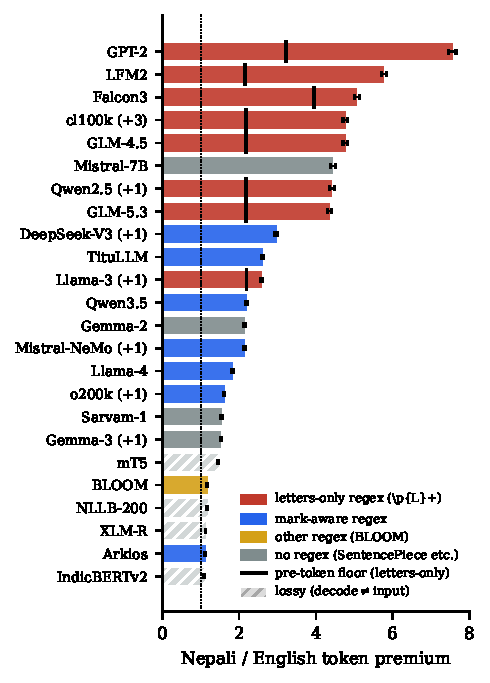
\includegraphics[width=0.95\columnwidth]{fig_audit.pdf}
\caption{Nepali/English token premium of 24 distinct tokenizers (33 released tokenizers; ``+$n$'' counts aliases) on FLORES-200 devtest, with 95\% paired-bootstrap intervals. Black ticks mark the pre-token floor of each letters-only tokenizer: no vocabulary extension can move its bar to the left of the tick.}
\label{fig:audit}
\end{figure}

\paragraph{Every letters-only tokenizer has a floor of at least $2.15\times$.} Eight distinct tokenizers, covering 13 released names including GLM-5.3 and LFM2, use the letters-only class. Their premiums range from $2.58\times$ (Llama-3) to $7.55\times$ (GPT-2), and their pre-token floors from $2.15\times$ to $3.23\times$. Excluding GPT-2, a 2019 model that we include as a historical reference, the premiums of current letters-only models range from $2.58\times$ to $5.77\times$ (LFM2). The seven lossless tokenizers with a mark-aware regex range from $1.12\times$ (Arkios;~\citealp{regmi2026arkios}) to $2.97\times$ (DeepSeek-V3).

\paragraph{Decomposition.} We write each premium as a product of three factors (Appendix~\ref{app:decomp}): a base term, which lies between $0.77$ and $0.80$ for every tokenizer; a \emph{regex factor}, the ratio of Nepali pre-tokens under the tokenizer's own regex to those under the repaired regex; and a \emph{vocabulary factor}, tokens per pre-token, which is the only factor vocabulary extension can lower, and only down to 1. The regex factor is $2.77$--$2.79$ for the Llama-3/Qwen/\texttt{cl100k} pattern, $4.06$ for the GPT-2 and Falcon3 patterns, and $0.98$--$1.02$ for mark-aware tokenizers. For Llama-3 the vocabulary factor is $1.18$, the lowest in the audit, so almost all of its remaining premium is the regex factor. Among mark-aware tokenizers it ranges from $1.43$ (Arkios) to $3.79$ (DeepSeek-V3): fixing the regex is necessary but not sufficient.

\paragraph{Within-family changes.} From Qwen3 to Qwen3.5 the Nepali premium halves ($4.42\times$ to $2.20\times$), with a word branch close to our repaired class~\citep{land2026smallbugs}; from Llama-3 to Llama-4, which adopts \texttt{o200k}'s pattern, it falls from $2.58\times$ to $1.83\times$. The vocabulary also grew in both cases, so these corroborate, but do not replace, the controlled comparison of \S\ref{sec:compression}.

\paragraph{Broken syllables.} Many Nepali tokens begin with a combining mark, which no well-formed Devanagari syllable does: 55\% of Llama-3's, and still 26\% of \texttt{o200k}'s, because BPE also splits within words (Appendix~\ref{app:audit}). \S\ref{sec:compression} shows how the rate moves under each retrofit.

\section{Pre-tokens bound merge-based extension}
\label{sec:floor}

A byte-level BPE tokenizer~\citep{sennrich-etal-2016-neural,radford2019language} first splits a string $s$ with a regex into pre-tokens $P(s)$ and then encodes each pre-token on its own by applying merges in rank order. Every pre-token yields at least one token, so $|T(s)| \ge |P(s)|$; \citet{regmi2026vowel} call this the pre-tokenization ceiling. Appending merges, whatever they are and however many, changes neither the normalizer nor the regex, so the bound holds for every tokenizer extended this way.

We turn this into a bound on the premium. For a tokenizer $T$ with pre-tokenizer $P$, the \emph{pre-token floor} is $|P(\text{ne})|/|T(\text{en})|$, the number of Nepali pre-tokens divided by the number of English tokens, summed over the 1{,}012 FLORES-200 devtest sentences. A merge-based extension that keeps $P$ and leaves English unchanged cannot bring the premium below this value, though it may stop above it. Our standard extension \RI{} leaves English unchanged: every new merge produces a token that contains a complete Devanagari code point, and since UTF-8 is self-synchronising, no new merge can fire on text without one (the same argument appears in the proof of Proposition~\ref{prop:lossless}, Appendix~\ref{app:proof}).

For today's regexes the floor is far from slack. In Llama-3 and Qwen the word branch is \texttt{[\textasciicircum\textbackslash r\textbackslash n\textbackslash p\{L\}\textbackslash p\{N\}]?\textbackslash p\{L\}+}, a run of letters optionally preceded by one other character. A Devanagari vowel sign ends the current run and becomes the leading character of the next one, so \emph{nep\=alko sark\=ar} (``government of Nepal'') becomes six pre-tokens, four of which start with a vowel sign that belongs to the previous consonant (Figure~\ref{fig:split}, Appendix~\ref{app:extras}). The floor is $2.19$ for Llama-3 and $2.17$ for Qwen3. That is above the premium of \texttt{o200k} ($1.61$), and 2.7 to 2.8 times the floor under the repaired regex of \S\ref{sec:method} ($0.79$ and $0.80$). Llama-3's premium is already $2.58$, so standard extension can lower it by at most 15\%.

\paragraph{Released extensions end at the floor.} Figure~\ref{fig:released} measures released merge-based extensions of letters-only models; Appendix~\ref{app:released} lists every number and how we found them. Ten extensions by Yamaguchi et al.\ of Llama-3, Llama-3.1, Qwen2.5 and Qwen3~\citep{yamaguchi2026lowres,yamaguchi2025elchat} cover six scripts written with combining marks. All ten end within 4\% of their floor, having closed at least 98\% of the distance from the base tokenizer.\footnote{These extensions re-order the base merges and change English token counts slightly (+6.5\% for the Llama-3 Telugu release), so for them we compare tokens with pre-tokens of the target text directly.} The 61k-token in-place expansion of LFM2 into LFM2.5~\citep{smith2026inplace} ends further from its floor ($1.07$ times it for Hindi, $1.16$ for Nepali, $1.24$ for Bengali and $1.82$ for Thai, which is written without spaces), but its floors are just as high. Under the repaired regex the same text has 2.2 to 5.9 times fewer pre-tokens, so each of these extensions stopped well short of what new vocabulary could achieve. Yamaguchi et al.'s Amharic extension, for a script without combining marks, stays at $1.57$ times its floor, and the repair does not change that floor.

\begin{figure}[t]
\centering
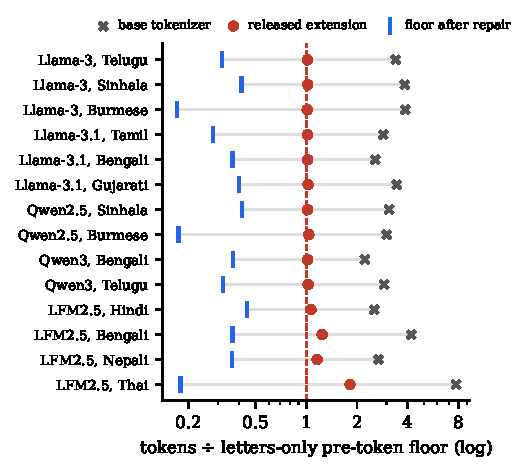
\includegraphics[width=0.95\columnwidth]{fig_released.pdf}
\caption{Released merge-based extensions of letters-only models on FLORES-200 devtest of each target language, relative to the letters-only pre-token floor. The ten extensions by Yamaguchi et al.\ (top) move from the base tokenizer ($\times$) to within 4\% of the floor (\textcolor{red}{$\bullet$}). LFM2.5 (bottom) stops further above it for Nepali, Bengali and Thai. The blue tick is the floor under the repaired regex. Full numbers, including the Amharic control, are in Table~\ref{tab:released}.}
\label{fig:released}
\end{figure}

\paragraph{Added tokens bypass the floor.} Strings registered as Hugging Face \emph{added tokens} are matched in the raw text before the regex runs, so the bound does not apply to them. SinLlama~\citep{aravinda2025sinllama} extends Llama-3 for Sinhala this way and goes below its letters-only floor. To test this route fairly, we registered as added tokens the 31{,}753 whole Devanagari strings among the 32{,}000 learned for \RII{} (\S\ref{sec:method}), on the unchanged regex. Nepali then costs $1.025$ times English on Llama-3 and $1.009$ on Qwen3, close to \RII{}'s $1.014$, and no FLORES-200 sentence without a Devanagari character changes its token ids. The floor therefore binds merge-based extension only. The price is the segmentation. Added tokens match the longest string anywhere, ignoring word boundaries, and 21\% of the matches start inside a word and 28\% end inside one. Allowing only whole-word matches (\texttt{single\_word=True}) removes those splits and also the gain: the premium returns to $2.49$ on Llama-3 and $4.22$ on Qwen3 (Appendix~\ref{app:extras}). We did not train models with added tokens.

\section{Repairing a deployed tokenizer}
\label{sec:method}

The repair has three parts: a one-class edit to the regex, new merges learned on top of the existing merge list, and an embedding initialisation that leaves the model's computation on old tokens unchanged.

\paragraph{Regex edit.} We admit \pM{} wherever the regex has a letter word class, and exclude it from the optional leading class and the punctuation class, so that a mark can only be matched by the word class and stays in one pre-token with the letters around it. For the Llama-3/Qwen pattern this is two substitutions (Appendix~\ref{app:regex}). Digits, contractions, whitespace and punctuation are handled as before. We call the result the \emph{repaired regex}. Qwen3.5 independently shipped almost the same word branch (\S\ref{sec:audit};~\citealp{land2026smallbugs}).

\paragraph{Continued BPE, restricted to Devanagari.} Following \citet{purason-etal-2026-teaching}, we learn $K$ new merges on top of the existing ones. We pre-tokenize Nepali text with the arm's regex, segment every pre-token with the \emph{original} merges, as the deployed model sees it, and run standard BPE over these segmentations, treating each base token as an indivisible symbol. We append the new merges after the existing ones, so the original merges act first at inference. We discard any merge whose output contains no code point in U+0900--U+097F, together with merges that depend on it. Two edge cases and implementation details are in Appendix~\ref{app:regex}. \RI{} and \RII{} use this identical procedure on identical text with identical $K$; they differ only in the regex.

\begin{proposition}[English invariance]
\label{prop:lossless}
Let $s$ be a string, after the tokenizer's normalizer, containing no code point of category \pM{} and no code point in U+0900--U+097F. Then the repaired tokenizer \RII{} and the original tokenizer produce identical token ids for $s$.
\end{proposition}
The proof is in Appendix~\ref{app:proof}. The proposition covers ASCII English and code, and every other script whose normalised text has no combining marks; it does not cover Devanagari or text with marks (Appendix~\ref{app:regex}).

\paragraph{Embedding initialisation.} Each new token's input and output rows are set to the mean of the rows of its constituent base tokens~\citep{gee-etal-2022-fast}, obtained by applying the original merges to its byte-level string. Original rows are untouched (Qwen3's first new tokens reuse its unused padding rows). On any input whose ids are all original, the resized model therefore gives the same logits for every original token as the base model; we check this on an English probe sentence (maximum absolute difference $<10^{-4}$). The softmax denominator gains the new tokens' logits, so continued pretraining is still needed.

\paragraph{Arms.} \RO{} (no extension) keeps the original tokenizer. \RI{} (extend) appends $K$ merges learned under the original letters-only regex: the standard recipe~\citep{purason-etal-2026-teaching,yamaguchi2026lowres}. \RII{} (repair + extend) switches to the repaired regex and appends $K$ merges learned under it. All arms then continue pretraining on the same bytes (\S\ref{sec:setup}).

\section{Experimental setup}
\label{sec:setup}

We registered the retrofit study in the project repository before training any model. A first amendment, committed before any continued-pretraining result, recorded our budget cuts and fixed the primary analysis. A second amendment, written after the first Llama results, added the warm-up runs described below, and a third, written before running it, added a Llama rerun with BOS in training. Appendix~\ref{app:prereg} gives all five commits and every deviation; details of training and evaluation are in Appendix~\ref{app:protocol}.

\paragraph{Models and data.} We use Llama-3.2-1B (base) and Qwen3-0.6B-Base, whose tokenizers ship the letters-only regex and which tie input and output embeddings. The Qwen3 tokenizer is identical across model sizes; we built it on Qwen3-1.7B-Base. Nepali text is FineWeb-2 \texttt{npi\_Deva} and English is FineWeb-Edu. We normalise to NFC, deduplicate, and remove every document that shares a whitespace 10-gram with FLORES-200 dev or devtest. A 30\,MB held-out slice of each language is never trained on. \RI{} and \RII{} learn merges on the same 1\,GB of Nepali, with the registered $K{=}32{,}000$.

\paragraph{Continued pretraining.} Each arm is trained for one epoch on the same documents, 1\,GB of Nepali and 1\,GB of English interleaved in one fixed order, with identical optimisation: a fixed, untuned peak learning rate of $10^{-4}$, cosine decay and one run per arm. Because \RII{} encodes the same bytes in fewer tokens, it takes fewer steps. \RO{} and \RI{} also save a checkpoint at the step where \RII{} ends, before their learning rate has decayed. We call these the \emph{main runs}. The \emph{warm-up runs} (Llama only) repeat them after first training only the embedding matrix on 10\% of the stream at a learning rate of $10^{-3}$.

\paragraph{Evaluation.} All metrics are normalised by UTF-8 bytes. The primary metric is bits per byte (BPB) on held-out native Nepali, \emph{byte-matched}: each document is split at whitespace into pieces of about 2{,}000 bytes, and every arm scores the same pieces. Each piece is scored after one context token. The \emph{registered prefix} is the beginning-of-sequence (BOS) token for Llama and the end-of-text token for Qwen, which has no BOS. In the main and warm-up runs, however, documents were separated only by the end-of-text token, so the Llama models never saw BOS. We therefore also score them after that token, the \emph{training separator}, as a diagnostic chosen after seeing results, and we reran the Llama main runs with BOS at every document start (\S\ref{sec:cpt}). Secondary metrics (held-out English BPB, FLORES BPB, Belebele, 5-shot translation) are in Appendix~\ref{app:cptfull}.

\paragraph{Analysis.} The registered main hypothesis was that \RII{} is non-inferior to both \RI{} and \RO{} on held-out Nepali BPB, with a margin of 0.01, while using fewer training tokens. The margin is 1.3\% of the base Llama model's Nepali BPB and 1.2\% of base Qwen's. We call \RII{} better if the 95\% interval of (\RII{} $-$ other) lies entirely below 0 and non-inferior if it lies entirely below $+0.01$. The first amendment called every other case ``no detectable difference''; the second split off ``worse'' for an interval entirely above 0, and we use that label because the first would misdescribe such an interval. The registered test was a paired bootstrap over held-out pieces. Pieces of one document are correlated, so we report a bootstrap over documents instead ($B{=}10{,}000$). Document ids were not stored with the pieces; we reconstruct them by taking a piece shorter than 1{,}900 bytes to end a document, which gives 484 Nepali documents from 2{,}259 pieces. On Nepali this widens the intervals by a factor of 1.3 to 2.3 and changes no verdict. The same test on English pieces is the registered English control. All intervals describe the sampling of evaluation text. With one run per arm, they say nothing about run-to-run variance.

\section{Results}
\label{sec:results}

\begin{table*}[t]
\centering\small
\setlength{\tabcolsep}{6pt}
\begin{tabular}{lcccc}
\toprule
 & \multicolumn{3}{c}{Llama-3.2-1B} & Qwen3-0.6B \\
\cmidrule(lr){2-4}\cmidrule(lr){5-5}
 & \multicolumn{2}{c}{main runs} & warm-up runs & main runs \\
\cmidrule(lr){2-3}\cmidrule(lr){4-4}\cmidrule(lr){5-5}
 & registered prefix & training separator & training separator & (both identical) \\
\midrule
\multicolumn{5}{l}{\emph{Held-out Nepali BPB} (lower is better)} \\
Base model, no training & 0.766 & n/a & n/a & 0.852 \\
\RO{} & 0.474 & 0.471 & 0.471 & 0.501 \\
\RI{} & 0.534 & 0.483 & 0.480 & 0.561 \\
\RII{} & 0.539 & 0.510 & 0.501 & 0.570 \\
\midrule
\multicolumn{5}{l}{\emph{Paired difference in held-out Nepali BPB} (positive: first arm worse), document-clustered 95\% interval} \\
\RI{} $-$ \RO{} & +0.060 & +0.012 & +0.010 & +0.060 \\
 & [+0.058, +0.061] & [+0.011, +0.013] & [+0.009, +0.011] & [+0.058, +0.062] \\[2pt]
\RII{} $-$ \RO{} & +0.066 & +0.039 & +0.031 & +0.070 \\
 & [+0.064, +0.068] & [+0.038, +0.041] & [+0.029, +0.032] & [+0.067, +0.072] \\[2pt]
\RII{} $-$ \RI{} & +0.006 & +0.027 & +0.021 & +0.009 \\
 & [+0.004, +0.007] & [+0.026, +0.028] & [+0.020, +0.022] & [+0.008, +0.010] \\
\midrule
Training tokens (M), \RO{}/\RI{}/\RII{} & \multicolumn{3}{c}{417 / 386 / 286} & 574 / 392 / 292 \\
Decoding steps, relative to \RII{} & \multicolumn{3}{c}{2.55 / 2.17 / 1} & 4.35 / 2.16 / 1 \\
\bottomrule
\end{tabular}
\caption{Continued pretraining on the same 1\,GB of Nepali and 1\,GB of English in every arm (one run per arm). BPB: bits per byte on held-out native Nepali, scored in pieces of about 2{,}000 bytes. Registered prefix: the beginning-of-sequence token, as pre-registered. Training separator: the end-of-text token that preceded every document during training (a post hoc diagnostic). Qwen has no beginning-of-sequence token, so both prefixes are the end-of-text token. Intervals resample 484 documents (2{,}259 pieces; a piece shorter than 1{,}900 bytes is taken to end a document) and reflect only the sampling of evaluation text. Warm-up runs under the registered prefix and all secondary metrics are in Table~\ref{tab:cpt}. Decoding steps: tokens needed for FLORES-200 Nepali devtest, relative to \RII{}.}
\label{tab:prefix}
\end{table*}


\subsection{Compression}
\label{sec:compression}

Figure~\ref{fig:ksweep} sweeps the number of new merges $K$. Under the letters-only regex (\RI{}), extension saturates almost at once. For Llama-3 the first 1{,}000 merges take the premium from $2.58$ to $2.32$, and the next 63{,}000 only to $2.20$, within $0.01$ of the floor. For Qwen3, \RI{} reaches $2.19$ by $K{=}16$k and stops at $2.18$, against a floor of $2.17$. It stops early because the letters-only regex leaves few distinct Nepali pre-tokens to merge (Appendix~\ref{app:extras}). Under the repaired regex (\RII{}), additional merges keep helping. At $K{=}32$k Nepali reaches parity with English ($1.01$) on both models, and at $64$k it is cheaper than English ($0.95$), below \texttt{o200k}. At $K{=}32$k, \RII{} needs 46\% of \RI{}'s tokens for FLORES Nepali. All 28 extended tokenizers decode losslessly and reproduce the original token ids on all 1{,}012 English devtest sentences, as \S\ref{sec:floor} and Proposition~\ref{prop:lossless} predict.

\begin{figure}[t]
\centering
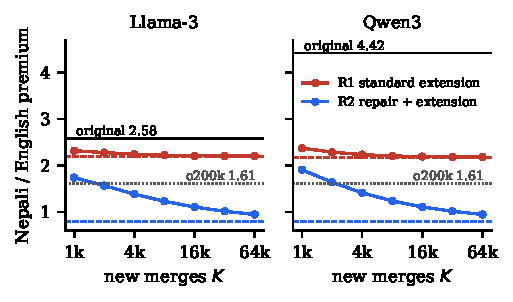
\includegraphics[width=\columnwidth]{fig_ksweep.pdf}
\caption{Nepali/English premium on FLORES-200 devtest after adding $K$ merges by continued BPE, under the letters-only regex (\RI{}) and the repaired regex (\RII{}). Dashed lines: pre-token floors under each model's own pattern ($2.19$ and $2.17$ letters-only; $0.79$ and $0.80$ repaired, for Llama-3 and Qwen3). 95\% paired-bootstrap intervals (half-width at most 0.03) are narrower than the markers.}
\label{fig:ksweep}
\end{figure}

Both parts of the repair are needed. Repairing the regex without new merges changes almost nothing ($2.61$ for Llama-3, $4.42$ for Qwen3), because the old merges still cut Nepali words into the old pieces. The repair also mends syllables. The share of Nepali tokens that start with a combining mark rises from 55\% (Llama-3) and 32\% (Qwen3) to 65\% and 64\% under \RI{}, since new merges can only build on mark-initial fragments, and falls to 13\% and 11\% under \RII{}.

We repeated the sweep for seven other languages written with combining marks and two controls (Table~\ref{tab:xling}, Appendix~\ref{app:xling}), learning merges on 25 to 361\,MB of FineWeb-2 text per language. At $K{=}32$k, \RII{} brings all seven to between $0.88$ and $1.24$ times English. \RI{} ends within 5\% of its floor in six of them. Thai is the exception: it is written without spaces, so its letters-only pre-tokens are long and leave \RI{} room. For Amharic and Korean, whose scripts have no combining marks, \RI{} and \RII{} are identical at every $K$, as the mechanism predicts.

\subsection{Continued pretraining}
\label{sec:cpt}

\paragraph{The registered outcome.} Table~\ref{tab:prefix} gives the results. The main hypothesis fails against \RO{}. Continued pretraining without new tokens gave the lowest held-out Nepali BPB on both models, and \RII{} was worse than \RO{} by $0.066$ on Llama and $0.070$ on Qwen, far beyond the 0.01 margin. Under this prefix standard extension also lost to \RO{}, by $0.060$ on both models. The new embeddings start as averages of existing ones, and 1\,GB of Nepali is not enough for them to catch up with tokens the base model already knows. Against standard extension, the registered comparison gives \RII{} $-$ \RI{} $= +0.0058$ $[+0.0044, +0.0073]$ for Llama, which is non-inferior, and $+0.0094$ $[+0.0084, +0.0104]$ for Qwen. The Qwen interval excludes zero and its upper end crosses the margin, so non-inferiority is not shown and \RII{} is worse. That verdict turns on 0.0004 BPB, a difference a second training run could plausibly move; we did not measure run-to-run variance.

\paragraph{The training separator.} For Llama, scoring after the training separator instead of BOS lowers BPB by $0.003$ for \RO{}, $0.051$ for \RI{} and $0.029$ for \RII{}, so the choice of first token changes the comparison. After the separator, \RII{} is worse than \RI{} by $+0.027$ $[+0.026, +0.028]$. We consider the separator scores closer to how the models were trained, but we chose them after seeing results, and BOS-prefixed inference is the default in Hugging Face and in chat templates, so the registered numbers are what a deployment would see. We have not established why the shift depends on the arm. With tied embeddings, the BOS row is updated as an output class even though it never appears as input, and in the warm-up runs its norm grows from $0.863$ to $0.896$ (Appendix~\ref{app:cptfull}); this may contribute. Training with BOS at every document start would remove the problem.

\paragraph{What the repair buys.} \RII{} trains on 26\% fewer tokens than \RI{} for the same bytes, but this does not make it cheaper to reach a given quality. At \RII{}'s final step count, the \RO{} checkpoint, whose learning rate had not yet decayed, is already better than the final \RII{} model by $0.060$ $[0.056, 0.063]$ on Llama and $0.053$ $[0.049, 0.057]$ on Qwen. The \RI{} checkpoint at that step is better by $0.006$ $[0.003, 0.008]$ on Llama and level on Qwen (scored on the first 1\,MB of held-out text, registered prefix). Measured training time fell by only 3\% (Llama) and 11\% (Qwen) relative to \RI{}, in runs that shared GPUs with evaluation jobs. The clear gain is at inference: for the same FLORES Nepali text, \RII{} needs $2.17$ (Llama) and $2.16$ (Qwen) times fewer decoding steps than \RI{}, which has the same vocabulary size, and $2.55$ and $4.35$ times fewer than \RO{}.

\paragraph{Warm-up runs.} Training only the embedding matrix first leaves \RO{} where it was ($0.471$ after the separator) and improves \RII{} from $0.510$ to $0.501$. \RII{}'s deficit relative to \RO{} shrinks from $0.039$ to $0.031$, as the second amendment predicted, and its gap to \RI{} from $0.027$ to $0.021$ $[0.020, 0.022]$. These are differences between single runs, so we treat them as suggestive. The amendment stated its prediction for the registered prefix, where the warm-up makes Llama scores unusable: \RO{} moves from $0.474$ to $0.779$.

\paragraph{English.} The registered English control holds. \RII{} $-$ \RO{} on held-out English is $+0.0003$ $[-0.0002, +0.0008]$ for Llama (non-inferior) and $-0.0028$ $[-0.0032, -0.0024]$ for Qwen (better), and no two main-run arms of a model differ by more than $0.004$. This is expected, since the tokenizer change does not touch English and every arm sees the same English data. Under the registered prefix all three Llama arms are slightly worse on English than the base model ($0.799$ to $0.803$ against $0.788$).

\section{Discussion}
\label{sec:discussion}

\paragraph{Recommendations.} Before extending a letters-only model (Table~\ref{tab:audit-full}) for a language with combining marks, compare the target text's pre-tokens with its tokens; our code includes a one-command check. If the two are close, as for Llama-3 on Nepali, merge-based extension has little room. At our budget, plain continued pretraining gave the best Nepali quality, so extension needs a reason beyond quality, such as inference cost. For that, we would use the Devanagari-only repair (untrained here, but identical to ours on FLORES Nepali), loaded with a class that does not rebuild its pre-tokenizer, and score models after the context they were trained with.

\paragraph{Why our sign differs from Regmi et al.} From scratch, the wider class lowers Nepali BPB by 4.4\%~\citep{regmi2026vowel}; retrofitted, it is worse than standard extension. A retrofit swaps known tokens for new ones initialised as averages and, at equal bytes, trains them for fewer steps, and extra steps explain most of an apparent Nepali pre-tokenization gain from scratch~\citep{shrestha2026papaya}. The from-scratch benefit may not come free in a deployed model.

\section*{Limitations}

\begin{itemize}
  \setlength\itemsep{0pt}
  \item \textbf{The main hypothesis failed.} At our budget, neither extension recipe beat continued pretraining without new tokens on Nepali BPB, and the repair scored below standard extension on both models, by a margin that training length may explain. Our evidence for the repair comes from compression and decoding cost only.
  \item \textbf{Scale.} We adapt 1B- and 0.6B-parameter models with 1\,GB of text per language and one epoch. The registered 3\,GB runs were dropped for budget reasons, so we cannot say whether the gap between arms closes with more data; \citet{dagan2024getting} needed more than 50B tokens to recover from a pre-tokenizer change.
  \item \textbf{Unequal training.} The registered design holds bytes fixed, so \RII{} takes 26\% fewer optimiser steps than \RI{} (545 against 737 for Llama), and Nepali falls from 45\% of \RI{}'s training tokens to 26\% of \RII{}'s. Part of the gap may come from \RII{} simply training less on Nepali. Our equal-compute checkpoints cut \RO{} and \RI{} short rather than training \RII{} longer, and the Llama ones carry the BOS artifact. We did not run \RII{} for as many steps as \RI{}.
  \item \textbf{Scoring one tokenization.} We score only the canonical tokenization of each piece. After extension, a model still assigns probability to the finer tokenizations of the base vocabulary, so the canonical score is a lower bound on its likelihood of the text, and the bound may be looser for \RI{} and \RII{} than for \RO{}, and for \RII{}, whose new tokens are longer, than for \RI{}. Marginalising over tokenizations~\citep{cao-rimell-2021-evaluate,chirkova-etal-2023-marginalize} would measure this; we did not.
  \item \textbf{One run per arm.} Every interval reflects only the sampling of evaluation text. We did not measure run-to-run variance, which is probably larger. Differences of a few thousandths, including the Qwen verdict against \RI{} and the warm-up effect, could change with another seed.
  \item \textbf{Approximate clustering.} Document boundaries in the evaluation set are reconstructed from piece lengths, so the clustered intervals are approximate.
  \item \textbf{Untuned optimisation.} One fixed learning rate ($10^{-4}$) is used for every arm; the registered learning-rate selection was not run. \RII{} takes fewer, larger steps than \RI{} and relies more on new embedding rows, so this recipe may handicap it. Mean initialisation may also suit \RII{}'s long new tokens less well than \RI{}'s short ones.
  \item \textbf{BOS in training.} The main and warm-up Llama runs never saw BOS, which the registered evaluation puts first, so their registered scores and all their secondary metrics carry this artifact; the warm-up translation scores are unusable. The rerun with BOS in training resolves the main comparison, but only on BPB: we did not run Belebele, translation or generation for it, nor a warm-up or equal-compute version. Qwen has no BOS token and was not affected.
  \item \textbf{Weak secondary metrics.} Belebele accuracy is near chance for every model, translation scores come from a single greedy pass without intervals and keep only the first output line, which is empty whenever a model begins its answer with a newline (we did not count how often), and measured generation speed was taken on shared GPUs (Appendix~\ref{app:cptfull}).
  \item \textbf{Equal compute.} The equal-compute checkpoints of \RO{} and \RI{} are taken before their learning rate has decayed, and are scored on 1\,MB only.
  \item \textbf{Languages.} We train models for Nepali only. For other languages we report compression, and the general repair, which we trained and released, changes the tokenization of 61 FLORES-200 languages whose quality we did not measure, including Hindi and Thai, which Llama 3.2 officially supports. The cross-script tokenizers use a relaxed merge filter not covered by Proposition~\ref{prop:lossless} (Appendix~\ref{app:xling}).
  \item \textbf{Added tokens and segmentation.} We measured the added-token route around the floor only at the tokenizer level and trained no model with it. Our objection to it is segmentation, and we have no evidence that segmentation matters for quality: our arms with more mark-initial tokens modelled Nepali better. Whether the regex repair beats added tokens is untested.
  \item \textbf{Scoring context.} The BOS-consistent rerun scores every piece after BOS, but 1{,}775 of the 2{,}259 pieces start mid-document, a context these models never saw after BOS in training.
  \item \textbf{What would settle it.} An \RII{} run with as many steps as \RI{}, three seeds per arm, a learning-rate sweep, annealed equal-compute runs and a curve over data budgets would show whether the gap between \RII{} and \RI{} comes from the tokenizer or from this recipe.
\end{itemize}

\section*{Ethics and use of AI assistance}

All text and evaluation data are public (FineWeb-2, FineWeb-Edu, FLORES-200, Belebele) and used under their licences; we collected no data from people. Released Llama-derived tokenizers follow the Llama 3.2 Community License~\citep{llama32license}; Qwen3-derived tokenizers are Apache-2.0.

We used a large language model assistant extensively. Under our direction it wrote and ran the experiment code, searched the literature and drafted the text. The author reviewed and approved the study design, the paper and all citations, and takes responsibility for the content. The numbers in the paper can be reproduced from public tokenizers and data with our released code.


\bibliography{refs}

\appendix
\section{Pre-registration history}
\label{app:prereg}

We pre-registered in four steps, in the public repository's git history, and report all four. Times are git commit times in IST (UTC+05:30).

\begin{enumerate}
  \setlength\itemsep{0pt}
  \item Commit \texttt{bf5ebe4} (2026-10-04 17:59 IST) registered hypotheses about the mechanism, a regex-only tokenizer ablation, a cross-script dose--response and from-scratch training. Our literature check then found that \citet{regmi2026vowel} had published the mechanism, the ablation, the cross-script analysis and a from-scratch downstream comparison five weeks earlier. We withdrew those hypotheses as contributions and do not report them as new.
  \item Commit \texttt{3c03367} (2026-10-04 18:16 IST), before any model was trained or evaluated, registered the retrofit study reported here: arms \RO{}, \RI{}, \RII{} and the untrained base model as a reference; $K{=}32{,}000$ unless \RII{} saturated earlier on FLORES dev; equal-bytes continued pretraining; learning rate selected once per model on \RO{}; two seeds; primary metric held-out native Nepali BPB with a non-inferiority margin of 0.01 bits per byte; English BPB as a control; Belebele, translation and decoding speed as secondary. Its compression prediction (P1), including the letters-only floors, had already been measured when it was written, so we report P1 as a measurement, not a confirmed prediction.
  \item Commit \texttt{5ff74e8} (2026-10-04 19:50 IST), amendment 2, was written after an internal review and before any continued-pretraining run had produced an evaluation. Earlier launches of continued pretraining were stopped by us before completion because of pipeline bugs, and none produced an evaluated checkpoint. The only evaluation run before the amendment, of the untouched base Llama-3.2-1B with a since-fixed document-prefix bug, is discarded. The amendment fixed the primary analysis as stated in \S\ref{sec:setup}.
  \item Commit \texttt{bfab80d} (2026-10-04 21:46 IST), amendment 3, was written \emph{after} observing Experiment A's Llama \RO{} and \RII{} results and before any \RI{} or Qwen result. It registered Experiment B (embedding warm-up, more data) and added a `worse' category to the claim rules. We report all comparisons under amendment 2's rules, which do not use that category.
\end{enumerate}

\paragraph{Deviations from the second registration (amendment 2).}
\begin{itemize}
  \setlength\itemsep{0pt}
  \item Qwen3-0.6B-Base replaces Qwen3-1.7B-Base (budget and time; same tokenizer).
  \item 1\,GB of Nepali and 1\,GB of English per arm replace 3\,GB and 3\,GB, with identical documents in every arm.
  \item A fixed learning rate of $10^{-4}$ for every run replaces selection on \RO{} from $\{3{\times}10^{-5}, 10^{-4}, 3{\times}10^{-4}\}$ by a 200-step pilot, which was never completed.
  \item One seed (seed 0) per arm replaces two.
  \item New: \RO{} and \RI{} are also checkpointed at \RII{}'s final step count (equal-compute view).
  \item New: byte-matched BPB on pieces of about 2{,}000 bytes is the primary metric; the registered sliding-window BPB becomes secondary.
  \item New: a paired bootstrap over held-out pieces, with explicit claim rules, is the primary test.
  \item The translation cap is 512 new tokens instead of 256, to avoid truncating Nepali output of \RO{}.
\end{itemize}

\paragraph{Pipeline bugs fixed before any reported run.} (1) Documents had been stored one per line with their internal newlines, so ``documents'' were paragraphs; they are now stored as one JSON-encoded document per line. (2) New-token embeddings had been initialised by decoding tokens to text, which turns partial UTF-8 tokens into U+FFFD; constituents now come from applying the original merges to the byte-level string. (3) The initialisation exactness check had covered Qwen's padding rows; it now covers only the original vocabulary. (4) Evaluation had prefixed documents with end-of-text, while base Llama expects its beginning-of-sequence token; we now use the latter where it exists, identically for every arm of a model.

Between the first two commits, the retrofit tokenizer code was tested on a 30\,MB sample of the FineWeb-2 Nepali \emph{test} split only.

\section{Repair details}
\label{app:regex}

\paragraph{Regex edit.} For the Llama-3/Qwen pattern the word branch changes as follows:
\begin{center}\small
\texttt{[\textasciicircum\textbackslash r\textbackslash n\textbackslash p\{L\}\textbackslash p\{N\}]?\textbackslash p\{L\}+}\\
$\downarrow$\\
\texttt{[\textasciicircum\textbackslash r\textbackslash n\textbackslash p\{L\}\textbackslash p\{M\}\textbackslash p\{N\}]?[\textbackslash p\{L\}\textbackslash p\{M\}]+}
\end{center}
and the same change is made in the punctuation branch \texttt{\textvisiblespace?[\textasciicircum\textbackslash s\textbackslash p\{L\}\textbackslash p\{N\}]+}. The optional leading class and the punctuation class must exclude \pM{}, so that a mark can only be matched by the word class and stays in one pre-token with the letters around it. Nothing else in the pattern changes.

\paragraph{Continued BPE.} At inference, BPE applies the lowest-ranked applicable merge first, so the original merges act before the new ones. The extended tokenizer reproduces the training procedure except in two cases: a new merge whose output string is already in the original vocabulary can let an original merge fire again afterwards, and under HuggingFace's \texttt{ignore\_merges} option (set for Llama-3) a pre-token that is itself a vocabulary entry is emitted directly. Neither case affects Proposition~\ref{prop:lossless}. We run the merge learning inside the HuggingFace Rust trainer by mapping each base token to a private-use code point. Learning $K{=}32{,}000$ merges on 1\,GB of Nepali text takes 1.7 to 3.4 minutes per tokenizer.

\paragraph{Scope of Proposition~\ref{prop:lossless}.} The proposition covers ASCII English and code, and every other script whose normalised text has no combining marks, including most Cyrillic, Han, Hangul and Ethiopic text. It does not cover Devanagari, even without marks: mark-free Devanagari words and Devanagari digits contain code points in U+0900--U+097F and change by design, since new merges apply to them. It also does not cover text with marks, such as Hindi or Latin written in decomposed form (NFD, e.g.\ \emph{caf\'e} with a combining acute). The Llama-3 tokenizer has no normalizer, so NFD input to a deployed Llama-3 \RII{} model falls outside the guarantee; Qwen3's tokenizer applies NFC itself, which composes most, but not all, combining marks. We normalise all our text to NFC. Empirically, \RI{} and \RII{} at $K{=}32{,}000$ give token ids identical to the original tokenizer on all 1{,}012 FLORES devtest sentences in English, Russian and Amharic, for both models. One Russian sentence contains a combining acute (U+0301) and so lies outside the proposition; its ids are nonetheless identical.

\paragraph{Embedding initialisation.} A new token's constituents come from applying the original merges to its byte-level string. We do not decode it to text, which would turn tokens ending in a partial UTF-8 sequence into U+FFFD. On any input whose ids are all original, the resized model produces the same hidden states, and the same logits for every original token, as the base model.

\section{Proof of Proposition~\ref{prop:lossless}}
\label{app:proof}

\begin{proof}
\emph{Pre-tokens.} The repaired regex differs from the original only in the three classes edited above, and each edited class differs from its original only on \pM{} characters. A regex match on $s$ consults only characters of $s$, and the order of the alternatives is unchanged. Since $s$ has no \pM{} character, both regexes produce the same pre-tokens.
\emph{Merges and vocabulary.} \RII{} differs from the original tokenizer only by appended merges and by the vocabulary entries they create, each of which contains a complete code point in U+0900--U+097F. A merge $(a,b)$ applies only where $a$ and $b$ are adjacent symbols of a pre-token, so its output is a contiguous substring of that pre-token's bytes. A vocabulary entry is emitted directly under \texttt{ignore\_merges} only if it equals the whole pre-token. Neither can happen for a pre-token of $s$, because UTF-8 is self-synchronising and $s$ contains no such code point. Each pre-token of $s$ is therefore encoded with original merges and original vocabulary entries only, exactly as by the original tokenizer.
\emph{Ids.} New ids are appended above the original ids, so all ids coincide.
\end{proof}

\section{Training and evaluation protocol}
\label{app:protocol}

\paragraph{Data.} We normalise to NFC, drop documents under 200 characters, remove exact duplicates, and drop every document that shares a whitespace 10-gram with FLORES-200 dev or devtest in Nepali or English. This also covers the Belebele passages, which are FLORES passages~\citep{bandarkar-etal-2024-belebele}, but not its questions or answers. Documents are stored one JSON-encoded document per line, so internal newlines are kept within a document. Before training, a 30\,MB held-out slice of each language is carved from the cleaned stream and never trained on. The 1\,GB of Nepali text used to learn merges is taken from the start of the training stream. Statistics are in Appendix~\ref{app:data}.

\paragraph{Continued pretraining.} Documents are interleaved by document and separated by the model's end-of-text token. We report each arm's training FLOPs. Optimisation is identical across arms: sequence length 2{,}048, global batch 256 sequences (0.52M tokens), AdamW ($\beta = (0.9, 0.95)$, weight decay 0.1), gradient clipping at 1.0, 1\% linear warm-up, then cosine decay to 10\% of peak, bf16 autocast with fp32 master weights, on 4$\times$H200. The peak learning rate is fixed at $10^{-4}$ for every run and is not tuned. Initialisation is deterministic and there is no dropout, so a second seed would change only the order of training windows and bf16 non-determinism.

\paragraph{Evaluation.} Every scored sequence is prefixed by the model's beginning-of-sequence token where it has one (Llama) and by its end-of-text token otherwise (Qwen), identically for every arm of a model. This is the registered prefix; \S\ref{sec:cpt} also reports a diagnostic re-scoring of held-out and FLORES BPB after the end-of-text token.
\begin{itemize}
  \setlength\itemsep{0pt}
  \item \textbf{Bits per byte (BPB)} on the held-out native Nepali and English slices (4\,MB each), and on FLORES-200 devtest. The primary metric is byte-matched BPB: each held-out document is split at whitespace into pieces of about 2{,}000 bytes, and every piece is scored independently, so every arm conditions on the same bytes of context. Token windows would give \RII{} more bytes of context per scored token. As a secondary metric, whole documents are scored with a sliding window of 2{,}048 tokens and stride 1{,}024.
  \item \textbf{Belebele}~\citep{bandarkar-etal-2024-belebele} \texttt{npi\_Deva} and \texttt{eng\_Latn}, zero-shot, scoring each of the four answer strings by its log-likelihood per byte given passage and question. Letter-choice prompting puts a 1B model at chance in both languages~\citep{regmi2026arkios}.
  \item \textbf{Translation}: FLORES-200 devtest Nepali$\leftrightarrow$English, 5-shot from FLORES dev, greedy decoding capped at 512 new tokens, chrF++.
  \item \textbf{Generation speed}: UTF-8 bytes generated per second in greedy continuation of FLORES dev Nepali sentences.
\end{itemize}
The equal-compute checkpoints are scored on BPB only, on the first 1\,MB of each held-out slice.

\section{Data}
\label{app:data}

\begin{table}[t]
\centering\small
\setlength{\tabcolsep}{3.5pt}
\begin{tabular}{lrr}
\toprule
& Nepali & English \\
\midrule
documents read & 170,790 & 215,961 \\
dropped: under 200 chars & 0 & 0 \\
dropped: exact duplicate & 0 & 69 \\
dropped: FLORES 10-gram & 0 & 16 \\
training documents & 166,300 & 209,713 \\
held-out (MB) & 30 & 30 \\
\midrule
\multicolumn{3}{l}{CPT tokens per arm (millions), 1\,GB + 1\,GB}\\
Llama-3.2-1B R0 & 207 & 211 \\
Llama-3.2-1B R1 & 176 & 211 \\
Llama-3.2-1B R2 & 76 & 211 \\
Qwen3-0.6B R0 & 359 & 215 \\
Qwen3-0.6B R1 & 177 & 215 \\
Qwen3-0.6B R2 & 76 & 215 \\
\bottomrule
\end{tabular}
\caption{Corpus cleaning (FineWeb-2 \texttt{npi\_Deva}; FineWeb-Edu; documents placed in the 30\,MB held-out slice are not counted as training documents) and the token counts of each arm's identical 2\,GB training stream. English token counts differ across arms of a model by less than 0.012\%, from the few English documents that contain Devanagari or combining marks.}
\label{tab:data}
\end{table}


\section{Full audit}
\label{app:audit}

Table~\ref{tab:audit-full} lists every distinct tokenizer. Aliases are tokenizers whose token counts are identical to another tokenizer's on all 36 FLORES languages we measured; we did not compare token ids. Kimi-K3 (requires executing remote code) and Mistral-Large-3 (degenerate HuggingFace load) are not included.

\begin{table*}[t]
\centering\small
\setlength{\tabcolsep}{4pt}
\begin{tabular}{lllrrrrrl}
\toprule
Tokenizer & Aliases & Regex & $|V|$ & ne/en & 95\% CI & Floor & Mark-init. & Lossless \\
\midrule
IndicBERTv2 & -- & none & 250,000 & 1.09 & [1.08, 1.10] & -- & 6\% & no \\
Arkios & -- & mark-aware & 65,536 & 1.12 & [1.10, 1.13] & 0.78 & 15\% & yes \\
XLM-R & -- & none & 250,002 & 1.12 & [1.11, 1.14] & -- & 7\% & no \\
NLLB-200 & -- & none & 256,204 & 1.17 & [1.16, 1.18] & -- & 6\% & no \\
BLOOM & -- & other & 250,680 & 1.18 & [1.16, 1.19] & -- & 17\% & yes \\
mT5 & -- & none & 250,100 & 1.46 & [1.45, 1.47] & -- & 11\% & no \\
Gemma-3 & Gemma-4 & none & 262,145 & 1.53 & [1.51, 1.54] & -- & 9\% & yes \\
Sarvam-1 & -- & none & 68,096 & 1.54 & [1.52, 1.56] & -- & 14\% & yes \\
o200k & gpt-oss & mark-aware & 200,019 & 1.61 & [1.60, 1.63] & 0.80 & 26\% & yes \\
Llama-4 & -- & mark-aware & 201,135 & 1.83 & [1.81, 1.85] & 0.80 & 30\% & yes \\
Mistral-NeMo & Sarvam-M & mark-aware & 131,072 & 2.13 & [2.11, 2.15] & 0.79 & 33\% & yes \\
Gemma-2 & -- & none & 256,000 & 2.13 & [2.11, 2.15] & -- & 19\% & yes \\
Qwen3.5 & -- & mark-aware & 248,077 & 2.20 & [2.18, 2.23] & 0.80 & 19\% & yes \\
Llama-3 & SmolLM3 & letters-only & 128,256 & 2.58 & [2.55, 2.61] & 2.19 & 55\% & yes \\
TituLLM & -- & mark-aware & 170,497 & 2.60 & [2.57, 2.63] & 0.78 & 55\% & yes \\
DeepSeek-V3 & DeepSeek-V4 & mark-aware & 128,815 & 2.97 & [2.93, 3.00] & 0.78 & 38\% & yes \\
GLM-5.3 & -- & letters-only & 154,856 & 4.35 & [4.29, 4.40] & 2.19 & 33\% & yes \\
Qwen2.5 & Qwen3 & letters-only & 151,665 & 4.42 & [4.36, 4.47] & 2.17 & 32\% & yes \\
Mistral-7B & -- & none & 32,768 & 4.44 & [4.38, 4.50] & -- & 29\% & yes \\
GLM-4.5 & -- & letters-only & 151,365 & 4.76 & [4.71, 4.82] & 2.19 & 30\% & yes \\
cl100k & Phi-4, OLMo-2, Granite-4.1 & letters-only & 100,277 & 4.76 & [4.71, 4.82] & 2.19 & 30\% & yes \\
Falcon3 & -- & letters-only & 131,072 & 5.07 & [5.00, 5.14] & 3.21 & 28\% & yes \\
LFM2 & -- & letters-only & 64,400 & 5.77 & [5.70, 5.84] & 2.15 & 24\% & yes \\
GPT-2 & -- & letters-only & 50,257 & 7.55 & [7.46, 7.65] & 3.23 & 19\% & yes \\
\bottomrule
\end{tabular}
\caption{All 24 distinct tokenizers (33 released tokenizers) on FLORES-200 devtest. Aliases: tokenizers with identical token counts on all 36 FLORES languages measured. Regex: letters-only, mark-aware, other, or none (no regex pre-tokenizer). ne/en: Nepali/English token premium with 95\% paired-bootstrap interval. Floor: pre-token floor under the tokenizer's own regex, a lower bound on the premium of any vocabulary extension (letters-only and mark-aware tokenizers only). Mark-init.: share of Nepali tokens whose first character is a combining mark. Lossless: decoding reproduces the input on 200 Nepali sentences. Arkios is from \citet{regmi2026arkios}. Hugging Face repositories are listed in the released code.}
\label{tab:audit-full}
\end{table*}


\paragraph{Broken syllables.} Many Nepali tokens begin with a combining mark, which no well-formed Devanagari syllable does: 55\% of Llama-3's Nepali tokens, 32\% of Qwen3's and 30\% of \texttt{cl100k}'s. The rate does not track the regex class. Mark-aware tokenizers show similar rates (26\% for \texttt{o200k}, 55\% for TituLLM, which keeps Llama-3's merges), because BPE also splits within words.

\section{Premium decomposition}
\label{app:decomp}

We write the premium as
\begin{equation*}
\frac{|T(\text{ne})|}{|T(\text{en})|} = \underbrace{\frac{|P_{\text{rep}}(\text{ne})|}{|T(\text{en})|}}_{\text{base}} \cdot \underbrace{\frac{|P(\text{ne})|}{|P_{\text{rep}}(\text{ne})|}}_{\text{regex factor}} \cdot \underbrace{\frac{|T(\text{ne})|}{|P(\text{ne})|}}_{\text{vocabulary factor}},
\end{equation*}
where $P$ is the tokenizer's own pre-tokenizer and $P_{\text{rep}}$ is the repaired Llama-3 pattern (\S\ref{sec:method}), applied to every tokenizer. The numerator of the base term is therefore the same for all tokenizers; only the English token count varies. The base lies between $0.77$ and $0.80$ for every tokenizer, because English token counts barely differ. The regex factor is $0.98$--$1.02$ for mark-aware tokenizers, $2.77$--$2.79$ for the Llama-3/Qwen/\texttt{cl100k} pattern, and $4.06$ for the GPT-2 and Falcon3 patterns, which put every run of marks in a pre-token of its own. The vocabulary factor, tokens per pre-token, is what vocabulary extension can lower, and only down to 1.

Table~\ref{tab:decomp} shows where each tokenizer's premium comes from. For Llama-3 the vocabulary factor is $1.18$, the lowest in the audit: its 128k vocabulary already nearly covers Nepali pre-tokens, and almost all of its remaining premium is the regex factor. For Qwen and \texttt{cl100k} both factors matter. Among mark-aware tokenizers, the vocabulary factor varies from $1.43$ (Arkios, trained for Nepali) to $3.79$ (DeepSeek-V3): fixing the regex is necessary but does not by itself make a tokenizer good at Nepali. Qwen3.5's word branch is our repaired class with only the leading-character class left unchanged; \citet{land2026smallbugs} reported its change for Hindi.

\begin{table}[h]
\centering
\small
\setlength{\tabcolsep}{4pt}
\begin{tabular}{lrrrr}
\toprule
Tokenizer & Premium & Base & Regex & Vocab. \\
\midrule
GPT-2 & 7.55 & 0.80 & 4.06 & 2.34 \\
LFM2 & 5.77 & 0.78 & 2.77 & 2.68 \\
\texttt{cl100k} (+3) & 4.76 & 0.79 & 2.77 & 2.17 \\
Qwen2.5/3 & 4.42 & 0.78 & 2.79 & 2.03 \\
GLM-5.3 & 4.35 & 0.79 & 2.77 & 1.98 \\
Llama-3 & 2.58 & 0.79 & 2.77 & \textbf{1.18} \\
\midrule
DeepSeek-V3/V4 & 2.97 & 0.80 & 0.98 & 3.79 \\
Qwen3.5 & 2.20 & 0.78 & 1.02 & 2.76 \\
Llama-4 & 1.83 & 0.80 & 1.00 & 2.30 \\
\texttt{o200k} (+1) & 1.61 & 0.80 & 1.00 & 2.01 \\
Arkios & 1.12 & 0.79 & 0.99 & 1.43 \\
\bottomrule
\end{tabular}
\caption{Premium = base $\times$ regex factor $\times$ vocabulary factor, on FLORES-200 devtest, for 11 of the 15 letters-only and mark-aware tokenizers in the audit (top: letters-only; bottom: mark-aware). Arkios is from \citet{regmi2026arkios}. Vocabulary extension can only lower the last column, and not below 1.}
\label{tab:decomp}
\end{table}

\section{Cross-script sweep}
\label{app:xling}

\begin{table}[h]
\centering
\small
\setlength{\tabcolsep}{3pt}
\begin{tabular}{lr|rrr|rrr}
\toprule
& & \multicolumn{3}{c|}{Llama-3} & \multicolumn{3}{c}{Qwen3} \\
Lang. & Marks & \RO{} & \RI{} & \RII{} & \RO{} & \RI{} & \RII{} \\
\midrule
Hindi & 31\% & 2.52 & 2.38 & 1.17 & 4.42 & 2.36 & 1.16 \\
Bengali & 32\% & 5.84 & 2.29 & 1.01 & 5.03 & 2.26 & 1.00 \\
Tamil & 35\% & 7.65 & 2.67 & 1.02 & 6.11 & 2.64 & 1.02 \\
Telugu & 36\% & 8.29 & 2.45 & 1.02 & 6.99 & 2.43 & 1.01 \\
Sinhala & 28\% & 8.63 & 2.30 & 1.20 & 6.88 & 2.33 & 1.24 \\
Burmese & 50\% & 11.62 & 3.02 & 1.21 & 8.93 & 2.99 & 1.11 \\
Thai$^\dagger$ & 21\% & 2.19 & 1.49 & 0.95 & 2.55 & 1.48 & 0.88 \\
\midrule
Amharic & 0\% & 7.59 & 0.98 & 0.98 & 4.05 & 0.98 & 0.98 \\
Korean & 0\% & 1.49 & 0.98 & 0.98 & 1.63 & 0.98 & 0.98 \\
\bottomrule
\end{tabular}
\caption{Language/English token premium on FLORES-200 devtest, $K{=}32{,}000$. Marks: share of NFC code points that are combining marks. Amharic and Korean have none (control). $^\dagger$Thai is written without spaces, so whole phrases are single pre-tokens and \RI{} is not yet at its floor. For \RI{}, merge learning stopped below 32{,}000 for Tamil, Telugu, Sinhala, Burmese and Hindi (Llama) (22{,}325--31{,}815 merges), because no further merge was available under the letters-only regex.}
\label{tab:xling}
\end{table}

For each language we downloaded the FineWeb-2 \emph{test} split, normalised it to NFC, and removed documents that share a whitespace 10-gram with that language's FLORES-200 dev or devtest (for Thai, which has no spaces, we also checked 50-character overlaps and found none). The resulting merge-learning text ranges from 25\,MB (Amharic) to 361\,MB (Bengali), less than the 1\,GB used for Nepali; Sinhala and Amharic \RII{} may be limited by it. $K{=}4$k and $16$k are prefixes of one $32$k run.

The Nepali filter keeps a new merge only if its output contains a complete Devanagari character. For scripts that the base vocabularies cover poorly, many characters are themselves split into byte pieces, and this filter would drop the first byte-level merge of a character and every merge built on it (for Sinhala \RII{}, on Llama-3, only 13{,}530 of 32{,}000 merges survived). For the cross-script sweep we therefore also keep merges whose output is a byte piece of a target-script character. Such merges can only fire on target-script bytes, so the English guarantee is unaffected; we verified English token ids on all 1{,}012 sentences for every tokenizer. Hindi uses the same script as Nepali, and its new merges also change Nepali tokenization; we did not measure that interaction.

\section{Released extensions}
\label{app:released}

\paragraph{Added tokens.} The bound does not apply to strings registered as HuggingFace \emph{added tokens}, which are matched before the regex runs. SinLlama~\citep{aravinda2025sinllama} extends Llama-3 for Sinhala this way, and thereby bypasses the bound for those exact strings. Added tokens are matched greedily and do not compose with merges, so they behave differently from a merge-based extension.

\begin{table}[h]
\centering
\small
\setlength{\tabcolsep}{3pt}
\begin{tabular}{llrrr}
\toprule
Base & Lang. & Tokens/floor & Gap closed & Room \\
\midrule
Llama-3-8B & te & 1.016 & 99.3\% & 3.16$\times$ \\
Llama-3-8B & si & 1.021 & 99.3\% & 2.42$\times$ \\
Llama-3-8B & my & 1.013 & 99.5\% & 5.87$\times$ \\
Llama-3.1-8B & ta & 1.018 & 99.1\% & 3.58$\times$ \\
Llama-3.1-8B & bn & 1.020 & 98.7\% & 2.74$\times$ \\
Llama-3.1-8B & gu & 1.026 & 98.9\% & 2.52$\times$ \\
Qwen2.5-7B & si & 1.019 & 99.1\% & 2.40$\times$ \\
Qwen2.5-7B & my & 1.036 & 98.2\% & 5.72$\times$ \\
Qwen3-14B & bn & 1.019 & 98.5\% & 2.71$\times$ \\
Qwen3-14B & te & 1.027 & 98.6\% & 3.11$\times$ \\
\midrule
LFM2 (2.5) & hi & 1.068 & 95.5\% & 2.24$\times$ \\
LFM2 (2.5) & ne & 1.160 & 90.5\% & 2.77$\times$ \\
LFM2 (2.5) & bn & 1.243 & 92.4\% & 2.74$\times$ \\
LFM2 (2.5) & th & 1.819 & 87.9\% & 5.57$\times$ \\
\midrule
Llama-3.1-8B & am & 1.573 & 93.8\% & 1.00$\times$ \\
\bottomrule
\end{tabular}
\caption{Released vocabulary extensions that keep the letters-only regex, on FLORES-200 devtest of the target language. Tokens/floor: extended-tokenizer tokens divided by pre-tokens under its own regex (at least 1 by construction). Gap closed: share of the base-to-floor gap that the extension removed. Room: floor under the letters-only regex divided by floor under the repaired regex. Top block: \citet{yamaguchi2026lowres}; middle: LFM2.5~\citep{smith2026inplace}; bottom: Amharic, which has no combining marks (control).}
\label{tab:released}
\end{table}

\section{Additional tokenizer arms}
\label{app:extras}

\paragraph{Regex alone, and added tokens.} Two further arms separate the parts of \RII{}. Repairing the regex without adding merges (\RII{}, $K{=}0$) changes almost nothing: $2.61\times$ for Llama-3 (from $2.58\times$) and $4.42\times$ for Qwen3. Under the repaired regex, the old merges still tokenize Nepali words in old pieces; the regex only removes the ceiling that new merges would otherwise hit. Registering \RI{}'s new strings (31{,}999 of 32{,}000; one is a partial UTF-8 sequence) as added tokens instead of merges gives $2.35\times$ for Llama-3 and $2.19\times$ for Qwen3, no better than \RI{}. The gain of \RII{} therefore needs both the regex repair and new merges.

\paragraph{Broken syllables.} Extension under the letters-only regex makes syllable breaking worse. The share of Devanagari-bearing tokens (a slightly higher base than the all-token rate of \S\ref{sec:audit}) that begin with a combining mark rises from 57\% (Llama-3) and 33\% (Qwen3) to 67\% for both under \RI{}, because new merges can only build on mark-initial fragments. Under \RII{} it falls to 15\% and 12\%.


\begin{figure}[h]
\centering
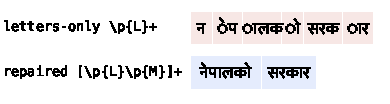
\includegraphics[width=0.95\columnwidth]{fig_split.pdf}
\caption{Pre-tokens of \emph{nep\=alko sark\=ar} (``government of Nepal'') under the letters-only regex of Llama-3 and Qwen and under the repaired regex. Dotted circles mark pre-tokens that begin with a dependent vowel sign.}
\label{fig:split}
\end{figure}

\section{All continued-pretraining runs}
\label{app:cptfull}

\begin{table*}[t]
\centering\small
\setlength{\tabcolsep}{4pt}
\resizebox{\textwidth}{!}{%
\begin{tabular}{lllrrrrrrrr}
\toprule
Model & Data & Arm & Tokens & ne BPB$\downarrow$ & en BPB$\downarrow$ & FLORES ne$\downarrow$ & Belebele ne & chrF ne$\to$en & chrF en$\to$ne & Gen.\ B/s \\
\midrule
Llama-3.2-1B & -- & base & 0 & 0.766 & 0.788 & 0.863 & 0.277 & 32.4 & 10.8 & 5327 \\
 & 1\,GB & \RO{} & 417M & \textbf{0.474} & 0.799 & 0.611 & 0.287 & 32.3 & 19.8 & 5147 \\
 & 1\,GB & \RI{} & 386M & 0.534 & 0.803 & 0.648 & 0.268 & 27.2 & 10.4 & 6354 \\
 & 1\,GB & \RII{} & 286M & 0.539 & 0.799 & 0.671 & 0.266 & 27.8 & 12.3 & 9398 \\
\addlinespace
 & 1\,GB + warm-up & \RO{} & 417M & 0.779 & 0.850 & 0.864 & 0.279 & 8.8 & 9.1 & 5349 \\
 & 1\,GB + warm-up & \RI{} & 386M & 0.808 & 0.854 & 0.904 & 0.271 & 9.9 & 4.2 & 7521 \\
 & 1\,GB + warm-up & \RII{} & 286M & \textbf{0.527} & 0.840 & 0.652 & 0.283 & 16.2 & 15.4 & 11078 \\
\addlinespace
\midrule
Qwen3-0.6B & -- & base & 0 & 0.852 & 0.873 & 0.945 & 0.290 & 26.0 & 6.8 & 2186 \\
 & 1\,GB & \RO{} & 574M & \textbf{0.501} & 0.864 & 0.631 & 0.270 & 20.1 & 13.6 & 3089 \\
 & 1\,GB & \RI{} & 392M & 0.561 & 0.864 & 0.689 & 0.253 & 11.6 & 6.9 & 4972 \\
 & 1\,GB & \RII{} & 292M & 0.570 & 0.862 & 0.688 & 0.266 & 17.0 & 3.9 & 7454 \\
\addlinespace
\bottomrule
\end{tabular}}
\caption{Continued pretraining on identical bytes per arm (one seed). BPB: bits per byte on held-out native text split into ${\sim}$2{,}000-byte pieces (primary metric) and on FLORES-200 devtest. Belebele: zero-shot accuracy (900 items, chance 0.25), scored on answer text. chrF++: 5-shot FLORES-200 devtest translation. Gen.\ B/s: UTF-8 bytes of Nepali generated per second (batch 64, greedy). Tokens: training tokens seen (for B1, excluding the embedding warm-up on the first 10\% of the same stream). Bold: best Nepali BPB within each block. All BPB here use the registered prefix; the B1 Llama rows are dominated by the scoring artifact of \S\ref{sec:cpt}, and Table~\ref{tab:prefix} gives the training-separator comparison.}
\label{tab:cpt}
\end{table*}


\paragraph{Beginning-of-sequence diagnostic.} On 40 held-out Nepali documents (first 1{,}500 characters), Llama BPB after the beginning-of-sequence token and after the end-of-text token are 0.720 and 1.865 for the base model, 0.441 and 0.438 for \RO{} of Experiment A, and 0.758 and 0.438 for \RO{} of Experiment B1. The norm of the beginning-of-sequence embedding is 0.863, 0.860 and 0.896 respectively (mean row norm 0.98--0.99).


\end{document}
